\def\SECTION{2.6 Proving Angle Relationships}
\documentclass[aspectratio=169,14pt]{beamer}
\usepackage[T1]{fontenc}
\usepackage{mathpazo}
\usepackage{amsmath,amssymb}
\usepackage{tikz}
\usetikzlibrary{arrows.meta,calc,decorations.pathreplacing}
\definecolor{fblue}{HTML}{1F4E79}
\definecolor{fteal}{HTML}{0F7C7C}
\definecolor{fgold}{HTML}{C9962B}
\definecolor{fred}{HTML}{B3261E}
\definecolor{fink}{HTML}{16233B}
\definecolor{fsoft}{HTML}{EEF3F8}
\definecolor{fgoldsoft}{HTML}{FBF1DC}
\setbeamertemplate{navigation symbols}{}
\setbeamercolor{normal text}{fg=fink}
\setbeamercolor{frametitle}{fg=fblue}
\setbeamerfont{frametitle}{series=\bfseries,size=\Large}
\setbeamercolor{structure}{fg=fteal}
\setbeamertemplate{itemize item}{\color{fteal}$\blacktriangleright$}
\setbeamertemplate{frametitle}{\vspace{6pt}\insertframetitle\par\vspace{-2pt}{\color{fgold}\rule{2.2cm}{2pt}}}
\setbeamertemplate{footline}{\hspace{0.6cm}{\color{fblue}\scriptsize\bfseries Fang\textcolor{fteal}{Math}}\hfill{\scriptsize\color{gray}\SECTION\quad\insertframenumber}\hspace{0.6cm}\vspace{6pt}}
\newcommand{\key}[1]{{\color{fteal}\textbf{#1}}}
\newcommand{\ans}[1]{\colorbox{fgoldsoft}{\color{fink}\ensuremath{#1}}}
\newcommand{\warn}[1]{\begin{beamercolorbox}[sep=8pt,rounded=true]{warnbox}{\color{fred}\textbf{Watch out!}}\enskip #1\end{beamercolorbox}}
\setbeamercolor{warnbox}{bg=fred!8,fg=fink}
\setbeamercolor{turnbox}{bg=fgoldsoft,fg=fink}
\setbeamercolor{defbox}{bg=fsoft,fg=fink}
\newcommand{\defn}[1]{\begin{beamercolorbox}[sep=8pt,rounded=true]{defbox}#1\end{beamercolorbox}}
\newenvironment{yourturn}{\begin{beamercolorbox}[sep=10pt,rounded=true]{turnbox}{\color{fgold}\Large\bfseries Your turn!}\quad{\small Pause the video and try it.}\par\medskip}{\end{beamercolorbox}}
\newcommand{\titleframe}[3]{%
\begin{frame}[plain]
\begin{tikzpicture}[remember picture,overlay]
\fill[fblue] (current page.north west) rectangle ([yshift=-0.9cm]current page.north east);
\node[anchor=west,text=white,font=\bfseries] at ([xshift=0.6cm,yshift=-0.45cm]current page.north west) {Fang\textcolor{fgold}{Math}};
\node[anchor=east,text=white,font=\small] at ([xshift=-0.6cm,yshift=-0.45cm]current page.north east) {Geometry $\cdot$ Chapter \CHNO};
\end{tikzpicture}
\vfill
{\color{fteal}\large\bfseries #1}\par\medskip
{\color{fblue}\fontsize{30}{34}\selectfont\bfseries #2}\par\medskip
{\color{fgold}\rule{3cm}{3pt}}\par\bigskip
{\large #3}
\vfill
{\small\color{gray} fangmath.com $\cdot$ YouTube @fangmathcom}
\end{frame}}
\newcommand{\closeframe}[1]{%
\begin{frame}{Remember}
#1
\vfill
\begin{center}{\color{fblue}\large\bfseries Now practice at your level:}\par\smallskip
{\Large\color{fteal}\bfseries fangmath.com} \enskip{\color{gray}$\to$ Geometry $\to$ Chapter \CHNO}\end{center}
\end{frame}}

\usepackage{pgfplots}\pgfplotsset{compat=1.17}
\newcommand{\grid}[4]{\draw[step=1,gray!25] (#1,#2) grid (#3,#4);\draw[-{Stealth},gray] (#1,0)--(#3+0.3,0) node[right]{\small$x$};\draw[-{Stealth},gray] (0,#2)--(0,#4+0.3) node[above]{\small$y$};}
\def\CHNO{2}
\usetikzlibrary{angles,quotes}
\begin{document}
\titleframe{Lesson 2.6}{Proving Angle Relationships}{Four facts you can use as reasons}
\begin{frame}{Four facts you can use}
\onslide<1->{\key{Linear Pair Postulate}: a linear pair is supplementary (adds to $180^\circ$).}\par\medskip
\onslide<2->{\key{Vertical Angles Congruence Theorem}: vertical angles are congruent.}\par\medskip
\onslide<3->{\key{Right Angles Congruence Theorem}: all right angles are congruent.}\par\medskip
\onslide<4->{\key{Congruent Supplements / Complements}: two angles supplementary (or complementary) to the \textbf{same} angle are congruent.}\par\medskip
\end{frame}
\begin{frame}{Why vertical angles are congruent}
\begin{columns}[c]\begin{column}{0.44\textwidth}\centering 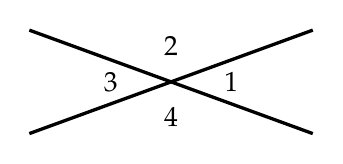
\begin{tikzpicture}[scale=0.9]\draw[very thick] (-2,-0.73)--(2,0.73); \draw[very thick] (-2,0.73)--(2,-0.73); \node at (0.85,0){$1$}; \node at (0,0.5){$2$}; \node at (-0.85,0){$3$}; \node at (0,-0.5){$4$};\end{tikzpicture}\end{column}\begin{column}{0.54\textwidth}\onslide<1->{$m\angle 1 + m\angle 2 = 180^\circ$ \hfill Linear Pair Postulate}\par\medskip
\onslide<2->{$m\angle 3 + m\angle 2 = 180^\circ$ \hfill Linear Pair Postulate}\par\medskip
\onslide<3->{$\angle 1 \cong \angle 3$ \hfill Congruent Supplements Theorem}\par\medskip
\onslide<4->{\defn{So vertical angles are congruent --- that's the whole proof.}}\par\medskip\end{column}\end{columns}
\end{frame}
\begin{frame}{Use it to find angles}
\begin{columns}[c]\begin{column}{0.44\textwidth}\centering 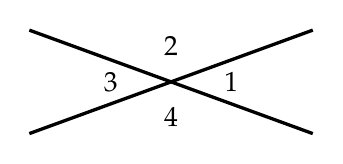
\begin{tikzpicture}[scale=0.9]\draw[very thick] (-2,-0.73)--(2,0.73); \draw[very thick] (-2,0.73)--(2,-0.73); \node at (0.85,0){$1$}; \node at (0,0.5){$2$}; \node at (-0.85,0){$3$}; \node at (0,-0.5){$4$};\end{tikzpicture}\end{column}\begin{column}{0.54\textwidth}\onslide<1->{$m\angle 1 = 3x + 10$, \quad $m\angle 3 = 5x - 30$}\par\medskip
\onslide<2->{Vertical angles are congruent: $3x + 10 = 5x - 30 \Rightarrow 40 = 2x \Rightarrow x = 20$}\par\medskip
\onslide<3->{$m\angle 1 = 3(20) + 10 = \ans{70^\circ}$, \quad $m\angle 2 = 180 - 70 = \ans{110^\circ}$}\par\medskip\end{column}\end{columns}
\end{frame}
\begin{frame}{Watch out}
\onslide<1->{\warn{Vertical angles are \textbf{across} from each other --- they are equal. Angles \textbf{next to} each other on a line are a linear pair --- they add to $180^\circ$, they are not equal.}}\par\medskip
\end{frame}
\begin{frame}{}
\begin{yourturn}$\angle A$ and $\angle B$ are both supplementary to $\angle C$. \\ $m\angle A = 2x + 15$, \quad $m\angle B = 3x - 5$. \ Find $x$ and $m\angle A$.\end{yourturn}\par\medskip
\onslide<2->{Congruent Supplements: $2x + 15 = 3x - 5 \Rightarrow x = \ans{20}$, \quad $m\angle A = \ans{55^\circ}$}\par\medskip
\end{frame}
\closeframe{\begin{itemize}\setlength\itemsep{8pt}
\item Linear pair: adds to $180^\circ$. \ Vertical angles: congruent.
\item All right angles are congruent.
\item Supplementary (or complementary) to the \textbf{same} angle $\Rightarrow$ congruent.
\end{itemize}}
\end{document}
